 \providecommand{\main}{../../..}
\documentclass[\main/main.tex]{subfiles}
\begin{document}
\subsection{Esercizio 3}

Si risolva mediante un algoritmo di Branch \& Bound il problema di zaino definito dai seguenti dati:

\begin{figure}
  \begin{subfigure}{0.31\textwidth}
    \[
      \bm{p} = \begin{bmatrix}
        16 \\
        14 \\
        12 \\
        9  \\
        10
      \end{bmatrix}
    \]
    \caption{Profitti}
  \end{subfigure}
  \begin{subfigure}{0.31\textwidth}
    \[
      \bm{w} = \begin{bmatrix}
        10 \\
        8  \\
        6  \\
        5  \\
        7
      \end{bmatrix}
    \]
    \caption{Pesi}
  \end{subfigure}
  \begin{subfigure}{0.31\textwidth}
    \[
      b = 18
    \]
    \caption{Capacità}
  \end{subfigure}
\end{figure}

Si utilizzi come rilassamento quello lineare, risolto mediante un opportuno algoritmo. Si rinominino gli indici delle variabili in base all’ordinamento ricavato.

Si adotti una strategia di esplorazione “Depth First ” e si esplori per primo, ad ogni livello, il ramo dell’albero di “branching” associato al vincolo xi = 1, dove la variabile di branching xi è quella che assume un valore frazionario nel rilassamento lineare.

Si noti inoltre che una variabile libera può venir fissata a zero qualora la capacità residua dello zaino sia strettamente minore del suo peso.

Si riporti a fianco l'albero di branching. Per ogni nodo si riportino: il suo numero progressivo, i (partendo dal valore 0 del nodo radice), il valore $UB_i$ ed il vettore con il corrispondente valore delle variabili.

\subsection{Risoluzione esercizio 3}

\subsubsection*{Costruisco modello}

\begin{figure}
  \begin{align*}
    \max_x z = \bm{p}^T \bm{x}                \\
    \bm{w}^T \bm{x} & \leq b                  \\
    x_i             & \in \crl{0,1} \forall x \\
  \end{align*}
  \caption{Modello dello zaino}
\end{figure}

\subsubsection*{Rilassamento lineare del modello}
\begin{figure}
  \begin{align*}
    \max_x z = \bm{p}^T \bm{x}                \\
    \bm{w}^T \bm{x} & \leq b                  \\
    x_i             & \in \sqr{0,1} \forall x \\
  \end{align*}
  \caption{Rilassamento lineare}
\end{figure}

\subsubsection*{Inizio algoritmo di Branch \& Bound}

\begin{enumerate}
  \item Ordino gli oggetti per valori non crescendi del rapporto $\frac{profitto}{volume}$.
  \item Associo all'oggetto $j-esimo$ il livello $j-esimo$ dell'albero.
  \item Al livello $j$ del ramo, genero due problemi figli:
        \subitem Primo: impongo che l'oggetto $j-esimo$ sia inserito.
        \subitem Secondo: impongo che l'oggetto $j-esimo$ non sia inserito.
  \item La regola di esplorazione è deep-first
\end{enumerate}

Prima di tutto calcolo la fitness per ogni oggetto:

\begin{figure}
  \begin{subfigure}{0.24\textwidth}
    \begin{align*}
      f(x_1) & = \sfrac{16}{10} = 1.6 \\
      f(x_2) & = \sfrac{14}{8} = 1.75 \\
      f(x_3) & = \sfrac{12}{6} = 2    \\
      f(x_4) & = \sfrac{9}{5} = 1.8   \\
      f(x_5) & = \sfrac{10}{7} = 1.4
    \end{align*}
    \caption{Fitness}
  \end{subfigure}
  \begin{subfigure}{0.24\textwidth}
    \begin{align*}
      x'_1 & = x_3 \\
      x'_2 & = x_4 \\
      x'_3 & = x_2 \\
      x'_4 & = x_1 \\
      x'_5 & = x_5
    \end{align*}
    \caption{Rimappamento}
  \end{subfigure}
  \begin{subfigure}{0.24\textwidth}
    \[
      \bm{p} = \begin{bmatrix}
        12 \\
        9  \\
        14 \\
        16 \\
        10
      \end{bmatrix}
    \]
    \caption{Profitti ordinati}
  \end{subfigure}
  \begin{subfigure}{0.24\textwidth}
    \[
      \bm{w} = \begin{bmatrix}
        6  \\
        5  \\
        8  \\
        10 \\
        7
      \end{bmatrix}
    \]
    \caption{Pesi ordinati}
  \end{subfigure}
  \caption{Riordino gli oggetti}
\end{figure}

Identifico \textbf{l'oggetto critico} al nodo radice, cioè l'oggetto il cui peso supera il limite massimo dello zaino: $6+5+8>b\rightarrow = 3$.

Identifico \textbf{l'upperbound di Dantzig} della radice, cioè il valore definito come:

\begin{figure}
  \[
    U = \floor{\sum_{j=1}^{s-1} p_j + \tilde{c}\frac{p_s}{w_s}}
  \]
  \caption{Upperbound di Danzig}
\end{figure}

In questo caso $U=33$.

\begin{figure}
  \begin{tikzpicture}
    \Tree[.$0:c=24,U=33$
      [.$x'_1=1$
          [.$1:c=18,U=33$
              [.$x'_2=1$
                  [.$2:c=7,U=33$
                      [.$x'_3=0$
                          [.$x'_4=0$
                              [.$x'_5=1$
                                  [.$3:\bm{x}=\sqr{1,1,0,0,1},z=31$ ]
                                ]
                            ]
                        ]
                    ]
                ]
                [.$x'_2=0$
                  [.$4:U=\floor{12+14+4\frac{16}{10}}=32$ ]
                ]
            ]
        ]
        [.$x'_1=0$
          [.$5:U=\floor{9+14+5\frac{16}{10}}=31$ ]
        ]
    ]
  \end{tikzpicture}
\end{figure}

La soluzione ottima ottenuta risulta essere quindi: $\bm{x}=\sqr{1,1,0,0,1}$, con $z=31$.

\end{document}